\documentclass[12pt]{article}

% French
\usepackage[utf8]{inputenc}
\usepackage[T1]{fontenc}
\usepackage[french]{babel}

\usepackage{hyperref}
\usepackage{pdfpages}
\usepackage{float}
\usepackage{geometry}
\usepackage{tikz}
\usepackage{eurosym}

\usepackage{multirow}

\usepackage{titlesec}

\titleformat*{\section}{\LARGE\bfseries}
\titleformat*{\subsection}{\Large\bfseries}
\titleformat*{\subsubsection}{\large\bfseries}
\titleformat*{\paragraph}{\large\bfseries}
\titleformat*{\subparagraph}{\large\bfseries}


\geometry{margin=2.5cm}

\definecolor{darkgreen}{RGB}{0,130,0}
\definecolor{darkblue}{RGB}{0,0,130}

\newcommand{\gameName}{Lands of Azerith}
\newcommand{\companyName}{Stonks Industries}
\newcommand{\progressbar}[1]{
    \begin{tikzpicture}
        \fill[black!30] (0,0) rectangle (#1/100*2cm, 0.2);
        \draw (0,0) rectangle (2cm, 0.2);
    \end{tikzpicture}
    \small{#1\%}
}


\title{
    Cahier des Charges \\
    \textbf{\gameName} \\
    \vspace{0.5cm}
    
\includegraphics[width=4cm]{format/logo.png}
    \vspace{4cm}
}
\author{
    Mohamed Aziz Ben Amor \\
    \texttt{mohamed-aziz.ben-amor@epita.fr}
    \vspace{0.5cm}\and
    Ayemane Bouarbi \\
    \texttt{ayemane.bouarbi@epita.fr}
    \vspace{0.5cm}\and
    Alexandre Cölsch \\
    \texttt{alexandre.colsch@epita.fr}
    \vspace{0.5cm}\and
    Michaël Museux \\
    \texttt{michael.museux@epita.fr}
    \vspace{0.5cm}\and
    Martin Pasquier \\
    \texttt{martin.pasquier@epita.fr}
}

\date{
    \vspace{1.5cm}
    \textbf{\companyName} \\
    \vspace{0.3cm}
    \textbf{EPITA} \\
    \vspace{1.5cm}
    \today
}

\begin{document}

\begin{titlepage}
    \maketitle
    \thispagestyle{empty} % Remove page number from title page
\end{titlepage}

\newpage
\thispagestyle{empty}
\mbox{}

\newpage
\tableofcontents

\newpage
\section{Introduction}

% En correction

Dans ce vaste monde qu’est le jeu vidéo, cinq étudiants débarquèrent de nulle part avec en tête une idée ambitieuse, créer de toutes pièces un jeu vidéo.
Dans une funeste atmosphère que représente une sombre salle machine de l’EPITA, très tard sous une nuit de pleine lune, fut créée la \textit{\companyName}.
Dans un but commun de devenir une des entreprises les plus prestigieuses dans ce monde, le premier jeu de la \textit{\companyName}, nommé \textit{\gameName}, vit le jour.
\\

\textit{\gameName} est avant tout un jeu vidéo de rôle se déroulant dans le monde médiéval fantastique de Stonkseria, qui est contrôlé par un régime impérial.
Le joueur aura le choix d’incarner plusieurs classes d’humains dans une faction indépendantiste et aura comme but de combattre l’empire en place et de le renverser, dans un monde où de nombreuses créatures malveillantes errent sans but dans la nuit.
\\

L'initiative autour de \textit{\gameName} découle de la demande du marché ainsi que de la validation du premier semestre, l’objectif principal est de développer un jeu captivant avec des graphismes de haute qualité pour assurer un engagement maximal des joueurs.
Sont impliqués dans ce projet les équipes de développement, d’art et de scénario, ainsi que les différents enseignants et jurys d’EPITA.
Ce cahier définit les exigences requises à la conception de ce jeu ainsi que les différentes échéances à venir.
Ces exigences comprennent des graphismes avancés, une jouabilité équilibrée sous Windows et le choix d’un moteur de jeu parmi la liste présentée par EPITA.
Par ailleurs, \textit{\companyName} s’engage à respecter les droits d’auteur pour les différentes ressources qui vont être utilisées.
La validation de ce cahier des charges sera assurée par les enseignants d’EPITA, et le suivi de ce jeu sera effectué lors de deux soutenances en 2024.
\\

Tout d’abord, ce document présentera le Cahier des Charges Fonctionnel (CdCF), qui se base sur les besoins fonctionnels du projet et la manière dont il sera traité sur le temps imparti.
Il se divise en plusieurs grandes catégories que sont les présentations de l’origine et du type du projet, des buts et intérêts ou encore des inspirations pour le projet, ainsi que la présentation de l’entreprise, la présentation de ses membres, la répartition des tâches et enfin un planning d’avancement des tâches.
Le projet aura à la fois un aspect fonctionnel, technologique, méthodologique et opérationnel, qui sera la structure même du CdCF.
\\

Enfin, ce dossier mettra en valeur le Cahier des Charges Technique (CdCT), qui détaille quant à lui les contraintes et les spécificités techniques nécessaires pour répondre aux besoins exprimés dans le cahier des charges fonctionnel.
Autrement dit, le CdCT détermine les moyens pour arriver à un résultat espéré sur le projet.
On y liste donc le choix des technologies, les exigences de performance, les critères d'acceptation, les exigences de compatibilité ou encore les caractéristiques techniques à respecter.





\newpage
\section{Cahier des Charges Fonctionnel}

\subsection{Origine et Nature du Projet}

% A corriger

\vspace*{0.2cm}

Le projet \textit{\gameName} est un jeu vidéo produit par le Studio \textit{Stonks Industries}. Il s’agit d’un RPG en 2D, en perspective du dessus. L’idée de ce projet nous est venue de grands classiques du jeu vidéo tels que les premiers opus de la licence \textit{Zelda}, ou encore de jeux plus récents comme \textit{Stardew Valley}, \textit{Cult of The Lamb} et \textit{Don’t Starve Together}. En effet, nous avons été séduit par l'expérience immersive que ces jeux ont à nous proposer, que cela soit en matière de jouabilité ou bien d’histoire, parfait pour la création d’un jeu vidéo au contenu riche et intéressant. 

C’est donc pour cela que nous nous sommes orientés vers la création d’un RPG en vue du dessus, dans un univers médiéval fantastique, idéal pour l’implémentation d’une histoire intrigante et remplie d’aventures. Cependant ce projet possèdera également sa propre identité ainsi que des mécaniques de jeu uniques tel que des cycles jour et nuits, la défense de base, ainsi que des assauts d’ennemis qui viendront ajouter du défis à l'expérience du joueur.

\subsubsection*{\hspace*{0.6cm}Description du projet}

Dans \textit{\gameName}, l'expérience immersive se déploie à travers le récit captivant d'un protagoniste plongé au cœur des terres énigmatiques de \textit{Stonkseria}. Émergeant au milieu de ruines celtiques, le joueur découvre rapidement un monde asservi sous le joug implacable d'un empire dictatorial. Animé par la soif de justice et de liberté, le personnage principal se dresse alors, armé de détermination et de courage, pour défier l'empereur déchu et libérer les villageois opprimés de l'emprise tyrannique qui les étouffe.
Cependant, le voyage du héros n'est pas sans embûches, car lorsque les ténèbres enveloppent la contrée, d'effroyables créatures surgissent des ombres pour entraver sa quête héroïque. Le joueur devra se préparer minutieusement pour affronter ces assauts nocturnes, érigeant des défenses solides pour protéger les zones vitales des attaques dévastatrices des forces maléfiques.
Au fil de cette aventure épique, le joueur devra prendre des décisions cruciales, forger des alliances stratégiques et maîtriser des compétences spéciales pour affronter les multiples défis qui jalonnent son périple. Avec des rebondissements narratifs captivants et des enjeux croissants, \textit{\gameName} promet une expérience de jeu riche en émotions et en défis, invitant les joueurs à plonger au cœur d'une quête légendaire pour la liberté et la justice.


Nous noterons également que \textit{\gameName} sera jouable en multijoueur, parfait pour créer des expériences  inoubliables entre amis .Les joueurs seront plongés dans une aventure immersive, alternant entre combats, quêtes, dialogues, et cinématiques, le tout en explorant une vaste carte regorgeant de mystères et de défis.

\subsubsection*{\hspace*{0.6cm}Style graphique}

En ce qui concerne le style graphique du projet, nous nous sommes orientés vers l’art du pixel étant donné que celui-ci se fond bien dans le style Médiéval fantastique. De plus, l’art du pixel est un style non seulement intemporel, mais il permet aussi la création relativement peu coûteuse de textures sans pour autant dégrader la qualité visuelle du projet. Nous noterons également que ce choix artistique peut potentiellement offrir une expérience plus nostalgique aux joueurs les plus anciens, ayant été habitués au graphisme des jeux arcades.

\subsection{Objet de l'\'Etude}

Le jeu \textit{\gameName}, représente bien plus qu'une simple initiative créative pour les membres de la \textit{Stonks Industries}. 
Il incarne une entreprise ambitieuse visant à apporter de l’innovation au sein de l'industrie du jeu vidéo, 
tout en offrant l'opportunité de développer des atouts majeurs pour chacun des membres de l’entreprise.
\\

% Buts :
L'objectif de cette étude est de présenter le projet de développement du jeu vidéo \textit{\gameName}.
Les objectifs fondamentaux qui ont façonné les fondements de ce projet captivant sont aussi variés qu'essentiels.
De prime abord, l'ambition de créer un jeu vidéo innovant et captivant se profile comme la base de ce projet.
Il s'agit de concevoir une expérience unique, en proposant aux joueurs une aventure immersive et inoubliable.
\\

Parallèlement, il est primordial de répondre aux attentes grandissantes de la communauté des joueurs, en offrant un gameplay riche et dynamique, un scénario complexe et captivant, ainsi que sa propre identité graphique, élevant ainsi les standards de qualité et d'engagement dans l'industrie.
Un autre objectif clé réside dans l'amélioration des compétences et des connaissances de l'équipe de développement, en encourageant la mise en place d’un environnement propice à l'apprentissage continu. 
L'implication dans ce projet servira de catalyseur pour l'acquisition de compétences techniques, ainsi que pour le renforcement des compétences interpersonnelles telles que la communication efficace, le leadership stratégique et la gestion agile des tâches complexes.
Enfin, tout en aspirant à la création d'une expérience ludique révolutionnaire, il est essentiel de garder un équilibre subtil entre l'innovation et la rentabilité. 
Le projet vise à garantir une gestion financière prudente et stratégique, veillant à ce que les investissements réalisés soient compensés par une valeur ajoutée significative pour l'entreprise.
\\

% Intérêts :
Sur le plan individuel, la participation active à ce projet ambitieux offre aux membres de l'équipe une occasion inestimable de cultiver leur talent et de cultiver une expertise solide dans le domaine complexe et en évolution constante du développement de jeux vidéo. 
Au-delà de l'aspect technique, le travail collaboratif et l'interaction fréquente avec des esprits créatifs et des passionnés du jeu encouragent l'acquisition de compétences cruciales telles que la communication, le leadership, ainsi que l'organisation méthodique des tâches complexes.
Sur le plan collectif, ce projet engendrera une dynamique de groupe propice à la construction d'une identité solide et d'une réputation enviable au sein de l'industrie. 
En outre, il s'agit d'une opportunité cruciale pour promouvoir le travail d'équipe de \textit{Stonks Industries}, en démontrant sa capacité à produire des jeux novateurs et captivants, ce qui, à son tour, peut catalyser l'acquisition de nouveaux contrats et l'expansion des opportunités commerciales.
\\

% Bénéfices potentiels :
Il ne faut pas sous-estimer les bénéfices lucratifs potentiels qui découlent de ce projet prometteur. 
En plus de l'enrichissement financier direct, le projet contribuera à l'élévation globale de la valeur de \textit{Stonks Industries} en tant qu'acteur majeur de l'industrie du jeu vidéo. 
Un jeu réussi renforcera non seulement la notoriété et l'influence de l'entreprise, mais attirera également l'attention d'investisseurs potentiels, ouvrant ainsi la voie à de nouvelles opportunités de croissance et d'expansion stratégique pour l'entreprise.



\subsection{\'Etat de l'Art}

Le genre du jeu de rôle (RPG) a une histoire riche et diversifiée, ayant évolué au fil des décennies pour offrir une multitude d'expériences immersives et captivantes aux joueurs du monde entier. 
Considéré comme l'un des genres les plus influents de l'industrie du jeu vidéo, le RPG a connu de nombreux titres à succès, dont certains ont marqué l'histoire du jeu vidéo.
\\

Le tout premier jeu de rôle notable, \textit{Dungeons \& Dragons} souvent abrégé D\&D, a jeté les bases du genre dans les années 1970 en popularisant les mécaniques de jeu de rôle basées sur le papier et le crayon.
En transportant les joueurs dans des mondes imaginaires remplis de quêtes épiques et de personnages fantastiques, D\&D a posé les fondations narratives et les mécanismes de jeu qui ont influencé de nombreux jeux vidéo de rôle ultérieurs.
\\

% Parmi les principaux jeux de rôle contemporains qui ont marqué l'industrie, trois titres notables incluent :

% \vspace{0.2cm}

% \begin{itemize}
%     \item \textit{Diablo} : Célébré pour sa réinvention du RPG avec le "point-and-click", ses graphismes réalistes et la qualité des modèles et animations, \textit{Diablo} envoie les joueurs dans un univers prenant et addictif.
%     Doté d'une i nterface simple à prendre en main et intégrant de la génération aléatoire de carte, le célèbre jeu a su apporter de la diversité et de la difficulté à ses joueurs. \\

%     \item \textit{The Elder Scrolls} : Acclamé pour son vaste monde ouvert et sa liberté de choix, \textit{The Elder Scrolls} offre aux joueurs la possibilité de façonner leur propre destinée dans un univers fantastique riche en aventures et en mystères.
%     Parmi ses caractéristiques notables figurent la personnalisation du personnage, les quêtes dynamiques et la possibilité de forger sa propre histoire. \\
    
%     \item \textit{Dark Souls} : Renommé pour son gameplay exigeant et sa conception de niveau complexe, \textit{Dark Souls} défie les joueurs avec des défis intenses et des combats stratégiques. Son atmosphère sombre et immersive, combinée à un système de combat gratifiant, a suscité l'admiration des joueurs passionnés de RPG exigeants.

% \end{itemize} 

% \vspace{0.5cm}

% Ces jeux de rôle remarquables se distinguent par leurs mondes captivants, leurs mécaniques de jeu uniques et leurs récits évocateurs, offrant aux joueurs des expériences inoubliables et une immersion profonde dans des univers riches et complexes. 
% \\

Étant l’une des licences majeures de Blizzard Entertainment \textit{Diablo}, a grandement façonné les jeux de rôle d'action qui lui ont succédé depuis ses débuts en 1996. 
Plongeant les joueurs dans un monde médiéval fantastique sombre et démoniaque, le jeu se distingue par son gameplay innovant axé sur l'exploration de donjons générés de manière procédurale, la collecte d'objets précieux , combat contre des créatures démoniaques et graphismes de grande qualité pour l’époque, le tout avec la possibilité de jouer en ligne avec d’autres joueurs. 
Avec son action frénétique et son emphase sur la recherche de trésors légendaires, \textit{Diablo} a rapidement gagné en popularité, établissant de nouveaux standards dans le genre des RPG d'action. 
La série, développée par \textit{Blizzard North}, a propulsé le concept de “hack 'n' slash”, où les joueurs peuvent améliorer leurs personnages en accumulant de l'expérience et en équipant des armes et armures de plus en plus puissantes, dans le but. 
La franchise a connu un succès commercial retentissant, avec plus de 2,5 millions d'exemplaires vendus dans le monde, confirmant ainsi sa position emblématique dans l'industrie du jeu vidéo.
\\

La suite The Elder Scrolls, avec son premier jeu publié en 1994 par \textit{Bethesda Softworks}, est la série de jeu de rôle et action la plus populaire du genre des RPG. 
Le dernier jeu de cette série, vendu à plus de 60 million de joueurs, \textit{The Elder Scrolls V} : \textit{Skyrim} est le plus populaire d'entre tous, sortant sur les nouvelles consoles plus de 10 ans après sa sortie en 2011. 
Bien que les jeux principaux sont tous en mode solo, \textit{The Elder Scrolls Online} propose du contenu en multijoueur. 
Une des raisons pour laquelle la série est si populaire est la liberté donnée au joueur, comme par exemple le choix du personnage et de sa race, ou la taille immense de la carte, ayant un total de 12 millions de km\^{2}. 
En effet, cela permet une immersion facile dans la peau de son personnage. 
L'ensemble de ces jeux sont aussi majoritairement basé sur un système de quêtes, qui guident le joueur lors de ses aventures.
\\

Une autre license de jeu de rôle majeure est \textit{Dark Souls}, constituée de trois jeux. 
Le premier jeu de la série est publié en 2011 par FromSoftware, et est suivi de \textit{Dark Souls} II et III en 2014 et 2016. 
Au premier abord, ce jeu n'est pas aussi populaire que ceux cités précédemment, mais il reste indéniablement l'un des jeux vidéo les plus influents. 
Les facteurs qui rendent ce jeu si intéressant sont les suivants. 
Tout d'abord, le gameplay en lui-même se démarque des autres jeux, en se concentrant sur la maîtrise de son personnage ainsi que ses armes et objets, ainsi que les mécaniques de combat. 
Ensuite, le level design pousse à l'exploration quasi constante pour découvrir le moindre passage secret, ainsi que l'histoire du jeu répartie çà et là pour laisser le joueur découvrir et même inventer sa propre histoire 

\subsection{Notre Entreprise}

\companyName est une entreprise qui est spécialisée dans le développement de jeux vidéo attractifs. 
Fondée par un groupe de cinq amis visionnaires et développeurs passionnés, Mohamed Aziz Ben Amor, Ayemane Bouarbi, Alexandre Cölsch, Michaël Museux et Martin Pasquier.
Guidée par l'esprit intrépide de ses fondateurs, l'entreprise s'est donnée pour mission de redéfinir l'expérience ludique grâce à des récits profonds, des visuels époustouflants et un gameplay engageant notamment grâce à leur jeu vidéo, \gameName, qui est en plein développement et cette entreprise a vu le jour dans une salle de l'EPITA, \companyName est née de la volonté de repousser les frontières de l'imaginaire et de l'innovation.
Basée à Paris, l'entreprise est reconnue pour son engagement à repousser les limites de la technologie et du gameplay et de créer des expériences immersives et captivantes pour les joueurs de tous âges. 
L'entreprise est dirigé par Mohamed Aziz Ben Amor, il en est le directeur général, pilote la vision stratégique de l'entreprise, mais aussi par Martin Pasquier qui est le directeur technique de l’entreprise qui lui canalise son perfectionnisme pour garantir que chaque produit soit à la pointe de la technologie.




La \textit{\companyName} est une entreprise spécialisée dans le développement de jeux vidéo depuis maintenant pr\`es de 1 mois.
Créée en 2023 par un groupe de cinq \'etudiants, cette derni\`ere s'est rapidement impos\'ee comme un leader dans l'industrie du jeu vidéo gr\^ace \`a sa passion pour l'innovation et la cr\'eativité. 
Basée à Paris, l'entreprise est reconnue pour son engagement à repousser les limites de la technologie et du gameplay afin de créer des expériences immersives et captivantes pour les joueurs de tous âges.
L'entreprise est dirig\'e par Mohamed Aziz Ben Amor, il en est le directeur général. 
\\

L'ambition autour du jeu \textit{\gameName} est \`a lier \`a son \'equipe d\'evou\'ee \`a cr\'eer des exp\'eriences innovantes, immersives et captivantes. 
L'équipe de développement de \textit{\gameName} est composée de 5 personnes, chacune ayant un rôle spécifique dans le développement du jeu.
\\

\subsubsection*{Gestion \'economique du projet}

Comme toute entreprise, la \textit{\companyName} a aussi des objectifs de rentabilité.
Estimer les co\^uts de développement du jeu, ainsi que les revenus potentiels est donc un enjeu majeur pour l'entreprise, afin d'assurer sa survie et sa croissance.
Le tableau ci-dessous (cf Figure \ref*{fig:couts_de_dev}) a pour objectif d'estimer les co\^uts de développement du jeu.
\\

\begin{figure}[H]
    \centering
    \begin{tabular}{|c|c|c|c|c|}
        \hline
        Cat\'egorie & Nom & Mois de travail & Montant Min & Montant Max \\
        \hline
        \multirow{3}{*}{\'Equipe de d\'eveloppement} & Développeurs C\# & 5 & 450 000 \euro  & 600 000 \euro \\
        \cline{2-5}
        & Game Designer & 5 & 35 000 \euro & 45 000 \euro \\
        \cline{2-5}
        & 2D Artist & 4 & 42 000 \euro & 50 000 \euro \\
        \hline
        Outils et logiciels & Licences logiciels & 5 & 5000 \euro & 7000 \euro \\
        \hline
        \multirow{2}{*}{Communication} & Site web & 2 & 10 000 \euro & 15 000 \euro \\
        \cline{2-5}
        & Marketing & 2 & 10 000 \euro & 15 000 \euro \\
        \hline
         & Serveurs de jeu & 8 & 80 000 \euro & 100 000 \euro \\




    \end{tabular}
    \caption{\'Estimation des co\^uts de développement du jeu}
    \label{fig:couts_de_dev}
\end{figure}






\subsection{Notre \'Equipe}

% A corriger

L'équipe de développement du projet est composée de 5 membres, tous étudiants à l'EPITA en classe de B1.
Chaques membres de l'équipe possède des compétences et des connaissances dans des domaines différents.
Cette polyvalence permet à l'équipe de répondre à tous les besoins du projet et de travailler de manière efficace et autonome.


\subsubsection*{Mohamed Aziz Ben Amor}

Aziz Ben Amor, âgé de 18 ans, est un élève dévoué à l'EPITA. 
Après avoir choisi des spécialités scientifiques axées sur l'informatique, il s'est inscrit à l'EPITA, une école renommée dans le secteur de l'informatique. 
Passionné par son domaine, il se consacre entièrement à la réussite de son parcours académique.
Cependant, ses intérêts ne se limitent pas à la programmation et au développement ; il est également fasciné par le monde de la finance et de l'entrepreneuriat. 
Il a acquis des connaissances en gestion d'entreprise, grâce à son intérêt pour ces sujets. 

D'origine tunisienne et ayant vécu en Tunisie pendant 18 ans, il maîtrise l'arabe maghrébin et possède une compétence modérée en anglais. 
Bien qu'il ait une maîtrise limitée de l'espagnol, il parle couramment le français, car il a été éduqué dans le système éducatif français.


% \newpage
\subsubsection*{Martin Pasquier}
    
Martin Pasquier est le directeur technique du projet, à l'age de 17 ans, il a déjà une bonne expérience dans le domaine de la programmation et du développement web.   
En tant que directeur technique, il est responsable de la gestion de l'équipe de développement et de la planification des tâches.
Il est également responsable de la conception et de la mise en œuvre du site web.

Sa passion pour la programmation ayant commencé à un age où le jeu vidéo était très présent dans sa vie.
Il  que Martin ai toujours voulu créer mon propre jeu vidéo.
De part son attrait pour la culture médiéval fantastique, il se prête aussi volontiers au role d'assistant au game designer, et il prend part à la conception du scenario et de l'histoire du jeu.

Martin est également un grand fan de musique, il aime écouter tout type de musique, ce qui lui sera utile pour la partie sonore du jeu.
La diversité de ses gouts musicaux lui permettra de créer une bande sonore riche et variée, qui s'adaptera parfaitement à l'ambiance du jeu.

\subsubsection*{Alexandre Colsch}

Alexandre Colsch a 17 ans et est étudiant en première année à l’EPITA.
Il est entre autres le cerveau derrière l’univers et l’histoire qui entoure le jeu.
Dès son plus jeune âge, il invente toute sortes d’histoires solides et détaillées, et depuis cette base solide de création d’histoires, Alexandre va mettre à profit son talent au service de Stonks Industries pour permettre aux jeux de l’entreprise d’avoir tout un univers très solide et un scénario digne des plus grands films Hollywoodiens.
Il a intégré l’EPITA pour mettre à profit sa passion pour l’informatique et la développer afin d’obtenir un très bon niveau en la matière.
Alexandre est également passionné par l’automobile et le sport automobile en général, éprouvant un très grand intérêt sur le sujet.
Sa passion se concrétise par ses bonnes performances en karting, sport qu’il adore faire mais il a très peu d'opportunités d’en faire.

Il est également un gros consommateur de jeux vidéos, un loisir qu’il aime faire et qu’il n'hésite pas à faire durant son temps libre.
Alexandre a intégré l'équipe de développement de Stonks Industries dès sa création et travaille sur le développement du premier jeu de l’entreprise dans le même but que tous les autres membres de l'équipe, créer son propre jeu vidéo.


\subsubsection*{Ayemane Bouarbi}

En tant que lead game artist, Ayemane, étudiant de génie a Epita, et à 18 ans seulement il se voit confier la lourde responsabilité de piloter la direction artistique du projet de jeu vidéo ambitieux “Land of Stonkseria”. 
Et ce choix n’a pas été realisé sans raison: Ayemane est un artiste du jeu vidéo ayant contruit sa propre réputation avec ses plus de 10 années d'expérience dans l’industrie. 
En effet, passionné par les jeux vidéo et de dessin depuis l’enfance, il commence à créer des jeux vidéo sur scratch dès l'âge de 7 ans avant de commencer à en faire sur python, et plus tard, en C++. 
Il a également de l’expérience dans la création de concepts art, la modélisation 3D, le texturing, le shading et le lighting.
Dans son parcours professionnel, il a participé à la direction artistique de plusieurs jeux vidéos, que cela soit avec de petits studios indépendants ou bien comme sur certains jeux classés AAA.
Dans son rôle actuel de Lead Game Artist chez les Studios Stonks Industries, il est responsable de la gestion et de la vision artistique du jeu, ainsi que de la  supervision de la création des assets et des textures du jeu.

\subsubsection*{Michaël Museux}

Michaël Museux, âgé de 17 ans, est étudiant à l'EPITA en première année de classe préparatoire intégrée. 

Depuis un très jeune âge, il est passionné par l'informatique, et plus particulièrement par la programmation.

Arès avoir découvert Scratch, il a par exemple écris des programmes pour résoudre des calculs complexes en mathématique, parfois même impossible à faire à la main.

Michaël est aussi passionné par l'algorithmie, son excellent niveau dans ce domaine lui a même permis de participer à des concours d'algorithmie, comme le concours Castor ou Algorea où il s'est classé parmi les meilleurs, alors qu'il n'était qu'au lycée. 

Attiré par l'idée de se faire ses propres outils, il s'est aussi intéressé à l’intelligence artificielle (IA) et notamment les technologies d’automatisation.
En effet, à une époque où la popularité des IAs grandissait de plus en plus, il semblait évident pour lui de s'y intéresser, et peut-être même d'en faire son métier.


Par coïncidence, Michaël intègre l'équipe de développement de \textit{\companyName}, qui commence le développement d'un nouveau jeu : \textit{\gameName}. 
Son rôle dans l'équipe est donc tout trouvé, il sera le développeur principal du jeu, avec un rôle important dans l'intelligence artificielle du jeu.
De plus, ses quelques compétences en développement web lui permettent de participer au développement du site web de l'entreprise.



\subsection{La Répartition des Tâches}

% Répartition : le cahier des charges doit contenir un planning détaillé de répartition des tâches par personne. 
% Vous le présenterez sous la forme d’un tableau à deux entrées (tâches, personnes) avec deux personnes par tâche : le responsable et son suppléant.


L'attribution des tâches est primordiale pour le bon déroulement du projet.
Chaque tâche est attribuée à un membre de l'équipe et il en est le responsable.
C'est son rôle de veiller à ce que la tâche soit bien réalisée dans les temps et qu'elle réponde au besoin pour laquelle elle a été créée.
Le responsable peut diviser sa tâche en sous-tâches et les attribuer à d'autres membres de l'équipe.
Cela lui permet de se concentrer sur sa tâche principale et d'arriver à un résultat plus rapidement.
\\

On assigne en plus un suppléant à celle-ci, qui pourra prendre le relais en cas d'indisponibilité du responsable.
En effet une tâche ne peut pas être laissée à l'abandon, elle pourrait mettre en retard tout le projet.
Ces rôles sont choisis en fonction des compétences de chacun, mais aussi en fonction de leurs disponibilités dans le projet.
Il est important de cerner les capacités des membres du groupe afin que leurs compétences soit utilisées au mieux.
\\

Les tâches sur le long terme (d'une durée supérieure à une semaine de travail)
sont listées dans le tableau ci-dessous (cf Figure \ref*{fig:repartition_des_taches}).
Il permet de voir qui est responsable de quelle tâche et de s'assurer que chaque tâche est bien assign\'ee à quelqu'un.
Ce tableau réunit les tâches par thèmes pour plus de lisibilité.


\begin{figure}[H]
    \centering
    \begin{tabular}{|c|c|c|c|}
        \hline
        \bfseries{Cat\'egorie} & \bfseries{T\^ache} & \bfseries{Responsable} & \bfseries{Suppl\'eant} \\
        \hline\hline
        % Général
        G\'en\'eral & Cahier des charges & Martin & Mohamed Aziz \\
        \hline\hline
        % Conceptualisation du jeu
        \multirow{2}{*}{Conceptualisation du jeu} & \'Ecriture du sc\'enario & Alexandre & Ayemane \\
        \cline{2-4}
        & \'Ecriture des dialogues & Ayemane & Mohamed Aziz \\
        \hline\hline
        % Site Web
        \multirow{3}{*}{Site Web} & Design du site web & Ayemane & Martin \\
        \cline{2-4}
        & Recherche technologie web & Martin & Michaël \\
        \cline{2-4}
        & Development du site web & Martin & Michaël \\
        \hline\hline
        % Texturing
        \multirow{2}{*}{Texturing} & Design des interfaces (UI) & Mohamed Aziz & Ayemane \\
        \cline{2-4}
        & Design personnages / terrains / objet & Ayemane & Alexandre \\
        \hline\hline
        % Intégration des textures
        \multirow{2}{*}{Intégration des Texturing} & Int\'egration des interfaces dans Godot & Mohamed Aziz &  \\
        \cline{2-4}
        & Int\'egration des textures dans Godot & Mohamed Aziz & \\
        \hline\hline
        % Level design
        \multirow{2}{*}{Level design} & Faire un schema de la carte & Alexandre & Mohamed Aziz \\
        \cline{2-4}
        &Level mapping avec les textures & Alexandre & Ayemane \\
        \hline\hline
        % Système d'équipements
        \multirow{3}{*}{Système d'équipements} & Listing items et objets (al\'eatoire) & Alexandre & Martin \\
        \cline{2-4}
        & Gestion al\'eatoire des objets & Alexandre & Martin \\
        \cline{2-4}
        & Equilibrage des objets & Alexandre & Martin \\
        \hline\hline
        % Multijoueur
        & Multijoueur & Mohamed Aziz & Michaël \\
        \hline\hline
        % IA
        \multirow{2}{*}{IA} & Pathfing des mobs & Michaël & Martin \\
        \cline{2-4}
        & Pathfing des mobs & Michaël & Martin \\
        \hline\hline
        % Musique et effet sonores
        & Musique et effet sonores & Ayemane & Martin \\
        \hline


    \end{tabular}
    \caption{R\'epartition des tâches}
    \label{fig:repartition_des_taches}
\end{figure}


Ce tableau présente les tâches sur le long terme, mais il est possible que des tâches plus courtes soient assignées à des membres de l'équipe.
Pour cela, nous avons fait le choix d'utiliser les outils proposés par GitHub.
En effet, les \textit{issues} permettent de lister les problèmes et les tâches à effectuer directement sur le dépôt du projet.
Cette intégration au plus proche du code permet de faciliter la gestion des tâches et la communication entre les membres de l'équipe.
\\






% Conceptualisation du jeu
    % Écriture du scenario
    % Écriture des dialogues

% Programmation
    % Proof of Concept / Test en Godot
    % Implémentation / Développement
    % Review / Debug / Publishing

% Site web
    % Design du site
    % Recherche technologie web
    % Développement du site
    
% Texturing
    % Réflexion sur le design globale (dessin)
    % Design des interfaces (UI)
    % Design personnages
    % Design terrains
    % Design objets

% Intégration des textures
    % Intégration des interfaces
    % Intégration des textures personnages
    % Intégration des textures terrains
    % Intégration des textures objets

% Level design
    % Faire un schema de la carte 
    % Level mapping avec les textures

% Système d'équipements
    % Listing items et objets (aléatoire)
    % Boutique (aléatoire) -> PNG et inventaire
    % Armurerie (aléatoire) -> Forgeron

% Mutlijoueur

% IA

% Musique et effet sonores




\subsection{Avancement et Planification}

% Avancement et planification : le cahier des charges doit contenir un planning détaillé d’avancement des tâches par période (temps séparant deux soutenances). 
% Vous le présenterez sous la forme d’un tableau à deux entrées (tâches, soutenances) avec un pourcentage d’avancement.

Afin de suivre l'avancement du projet, nous avons listé les tâches importantes du projet et nous en avons fait un planning prévisionnel.
Dans le tableau ci-dessous (cf Figure \ref*{fig:avancement_planification}), on trouve le pourcentage d'avancement de chaque tâche pour chaque soutenance.
Il s'agit donc de synthétiser nos objectifs pour chaque soutenance.
\\

Comme tous les projets, il n'est pas impossible que nous rencontrions des problèmes qui pourraient retarder le développement du jeu.
Avoir un planning fixé dès le début du projet permet de se fixer des objectifs et de pouvoir les atteindre.
Il permet aussi de tester la faisabilité de chaque tâche dans le temps imparti et de pouvoir réagir rapidement en cas de dépassement de la durée allouée.
\\

\begin{figure}[H]
    \centering
    \begin{tabular}{|c|c|c|c|}
        \hline
        Tache & 1\up{\'ere} soutenance & 2\up{ème} soutenance & 3\up{ème} soutenance \\
        \hline
        Site web & + & ++ & +++ \\
        \hline
        Concept du jeu & +++ & +++ & +++ \\
        \hline
        Design des textures & + & ++ & +++ \\
        \hline
        D\'eveloppement du jeu dans godot &  & ++ & +++ \\
        \hline
        Multijoueur &  & ++ & +++ \\
        \hline
        Musique et effets sonores &  & + & +++ \\
        \hline
    \end{tabular} \\
    \vspace*{0.2cm}
    + : Tâche non commencée  /  ++ : Tâche en cours  /  +++ : Tâche terminée\\

    \caption{Répartition des tâches}
    \label{fig:avancement_planification}
\end{figure}







\subsection{Le choix des technologies}

Le language de programmation C\# semble est le plus adapté pour le développement de \textit{\gameName}. 
Dérivée du C++ et étonnamment proche du \textit{Java}, Il permet de coder des jeux vidéos grâce à sa compatibilité avec les moteurs de jeu \textit{Godot} ou encore \textit{Unity}.
Nous utiliserons l’environnement de développement intégré (IDE) \textit{Rider} proposé par \textit{JetBrains}, qui  nous permettra d’avoir à disposition tous les outils nécessaires pour coder notre projet du début à la fin.
\\

Ensuite, pour les textures graphiques du jeu, nous utiliserons le logiciel de retouche \textit{Adobe Photoshop}, qui nous permettra donc de traiter les différents environnements, les différentes textures au sein du jeu et tout ce qui touche les graphismes en général.
Ce sera sans doute le logiciel principal du directeur graphique du groupe, c'est un outil très complet et très puissant qui répondra à tous ses besoins.
\\

Puis, nous utiliserons principalement \textit{GitHub} comme environnement de travail, qui est est un service web d’hébergement et de gestion de développement de logiciels, utilisant le logiciel de gestion de versions \textit{Git}. 
L’utilisation de \textit{GitHub} nous permettra de mettre en commun nos tâches et de les réunir dans notre projet global, en guise d’exemple, un membre du groupe qui doit fournir un code pour un autre membre peut directement passer par \textit{GitHub} pour lui fournir, ou encore deux membres qui ont la même tâche peuvent travailler et modifier le code en même temps grâce au dépot \textit{Git}, et ainsi travailler plus efficacement.
\\

En plus de cela, notre groupe utilisera le logiciel de messagerie instantanée \textit{Discord} pour essentiellement communiquer sur l’avancée du projet, mais aussi partager l’avancement de chacun sur ses tâches ou encore s’organiser sur les prochaines tâches du projet. Tout cela peut se résumer en de brèves discussions jusqu’à des réunions en appel vocal qui peuvent durer un certain temps rendant la répartition des différentes tâches efficace.
\\

Nous utiliserons aussi le moteur de jeu multiplateforme \textit{Godot} pour la création de notre jeu vidéo.
Il contient tout ce dont on aura besoin pour le développement de \textit{\gameName}, comme le moteur 2D, le moteur physique, un gestionnaire d’animations ou encore des langages de script pour la programmation des comportements. 
Comme cité précédemment, c’est avec le langage C\# que l’on utilisera le moteur \textit{Godot}, afin de mener à bien notre projet.
\\

Enfin, au niveau du matériel, nous utiliserons chacun nos pc personnels pour avancer sur les tâches et les projets depuis chez soi, mais nous aurons également à disposition et utiliserons par ailleurs les pc des locaux de la \textit{Stonks Industries}, situés en salles machines de l’EPITA, qui nous permettra de travailler directement sur place avec un environnement purement professionnel.
\\


\section{Cahier des Charges Technique}

Les deux prochaines pages sont dédiées au cahier des charges technique.
Ce document détaille les contraintes et les caractéristiques techniques nécessaires pour répondre aux besoins du projet.
Il synthétise toutes les réponses aux questions techniques que l'on peut se poser sur le projet.
\\

Le cahier des charges technique est divisé en deux parties.
La première partie détaille les spécificités du jeu et les choix techniques qui ont été réalisés. 
La deuxième partie donne des informations sur la repartition des tâches et leur avancement.


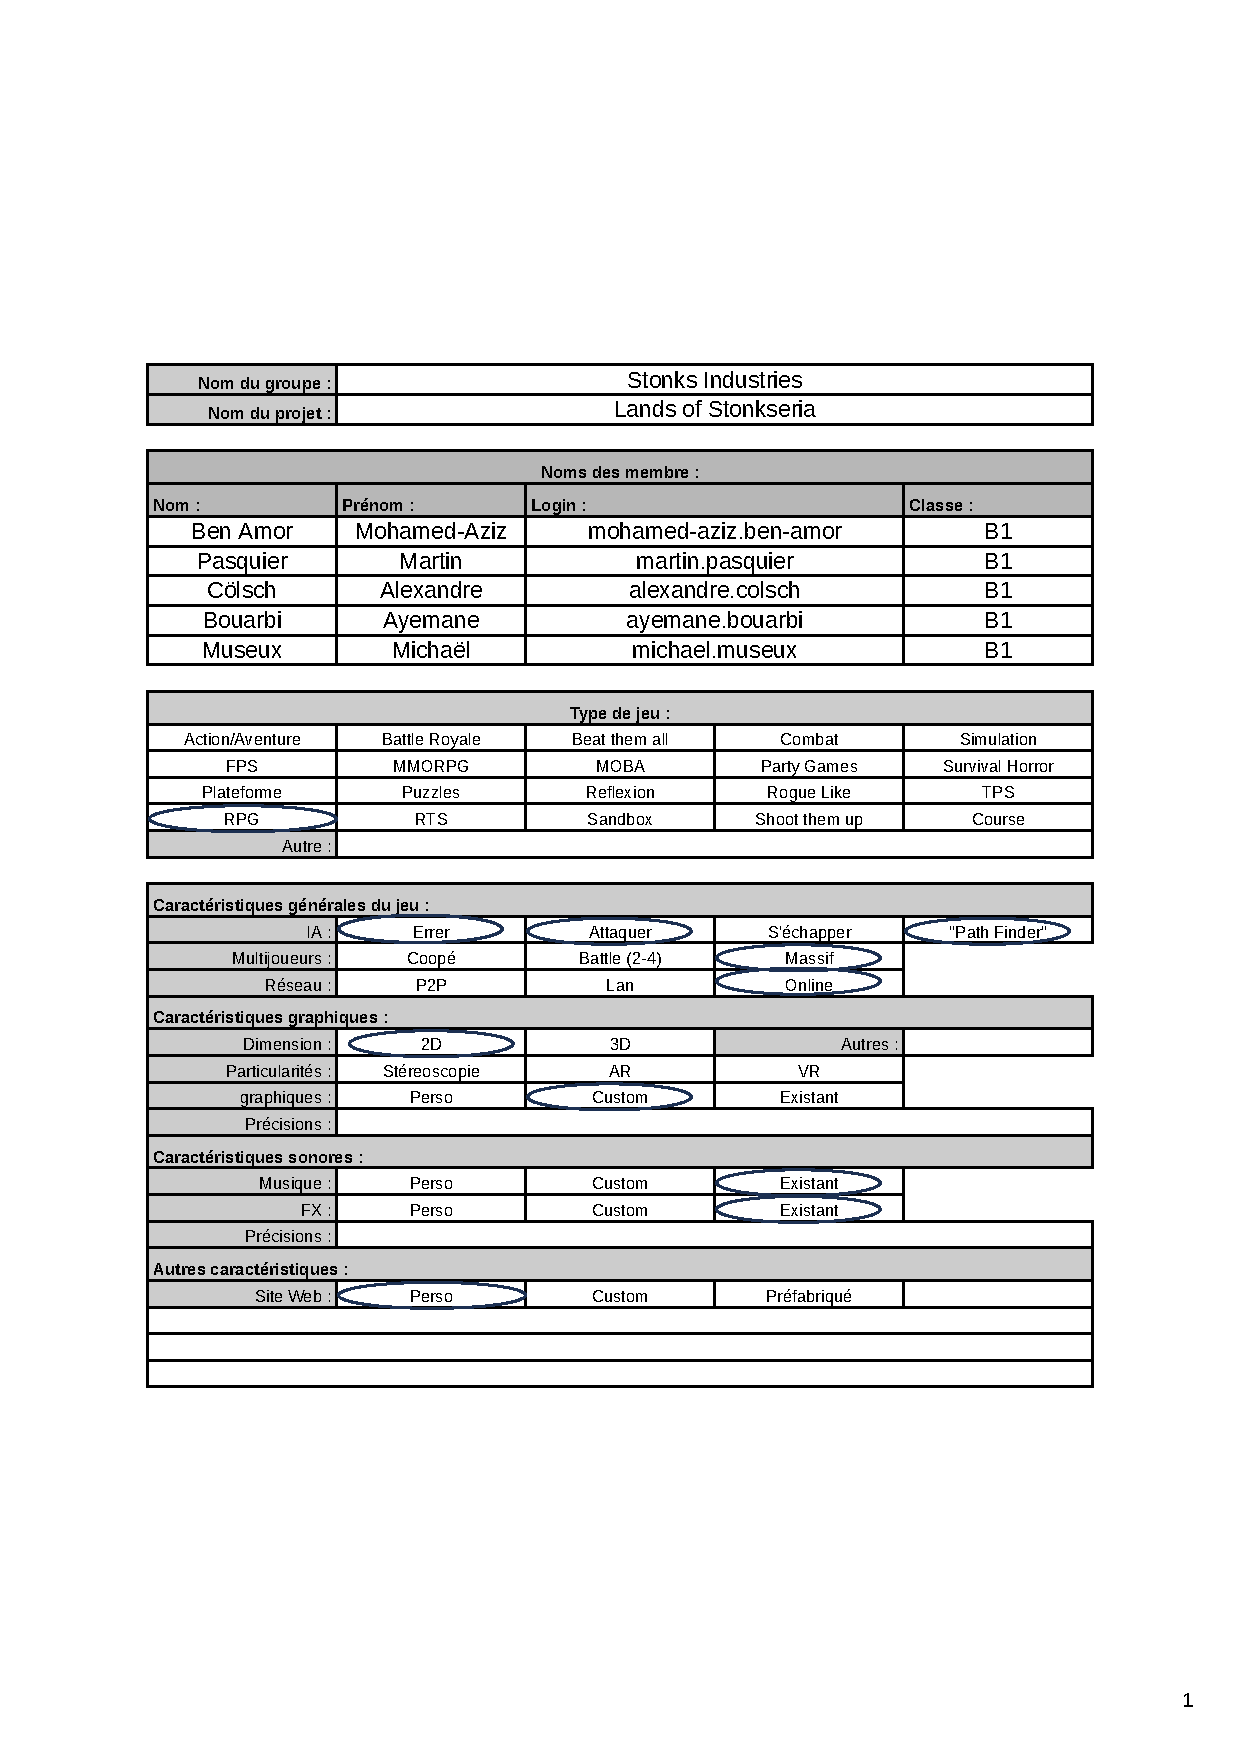
\includepdf[pages=1]{format/Technical_book-1.pdf}

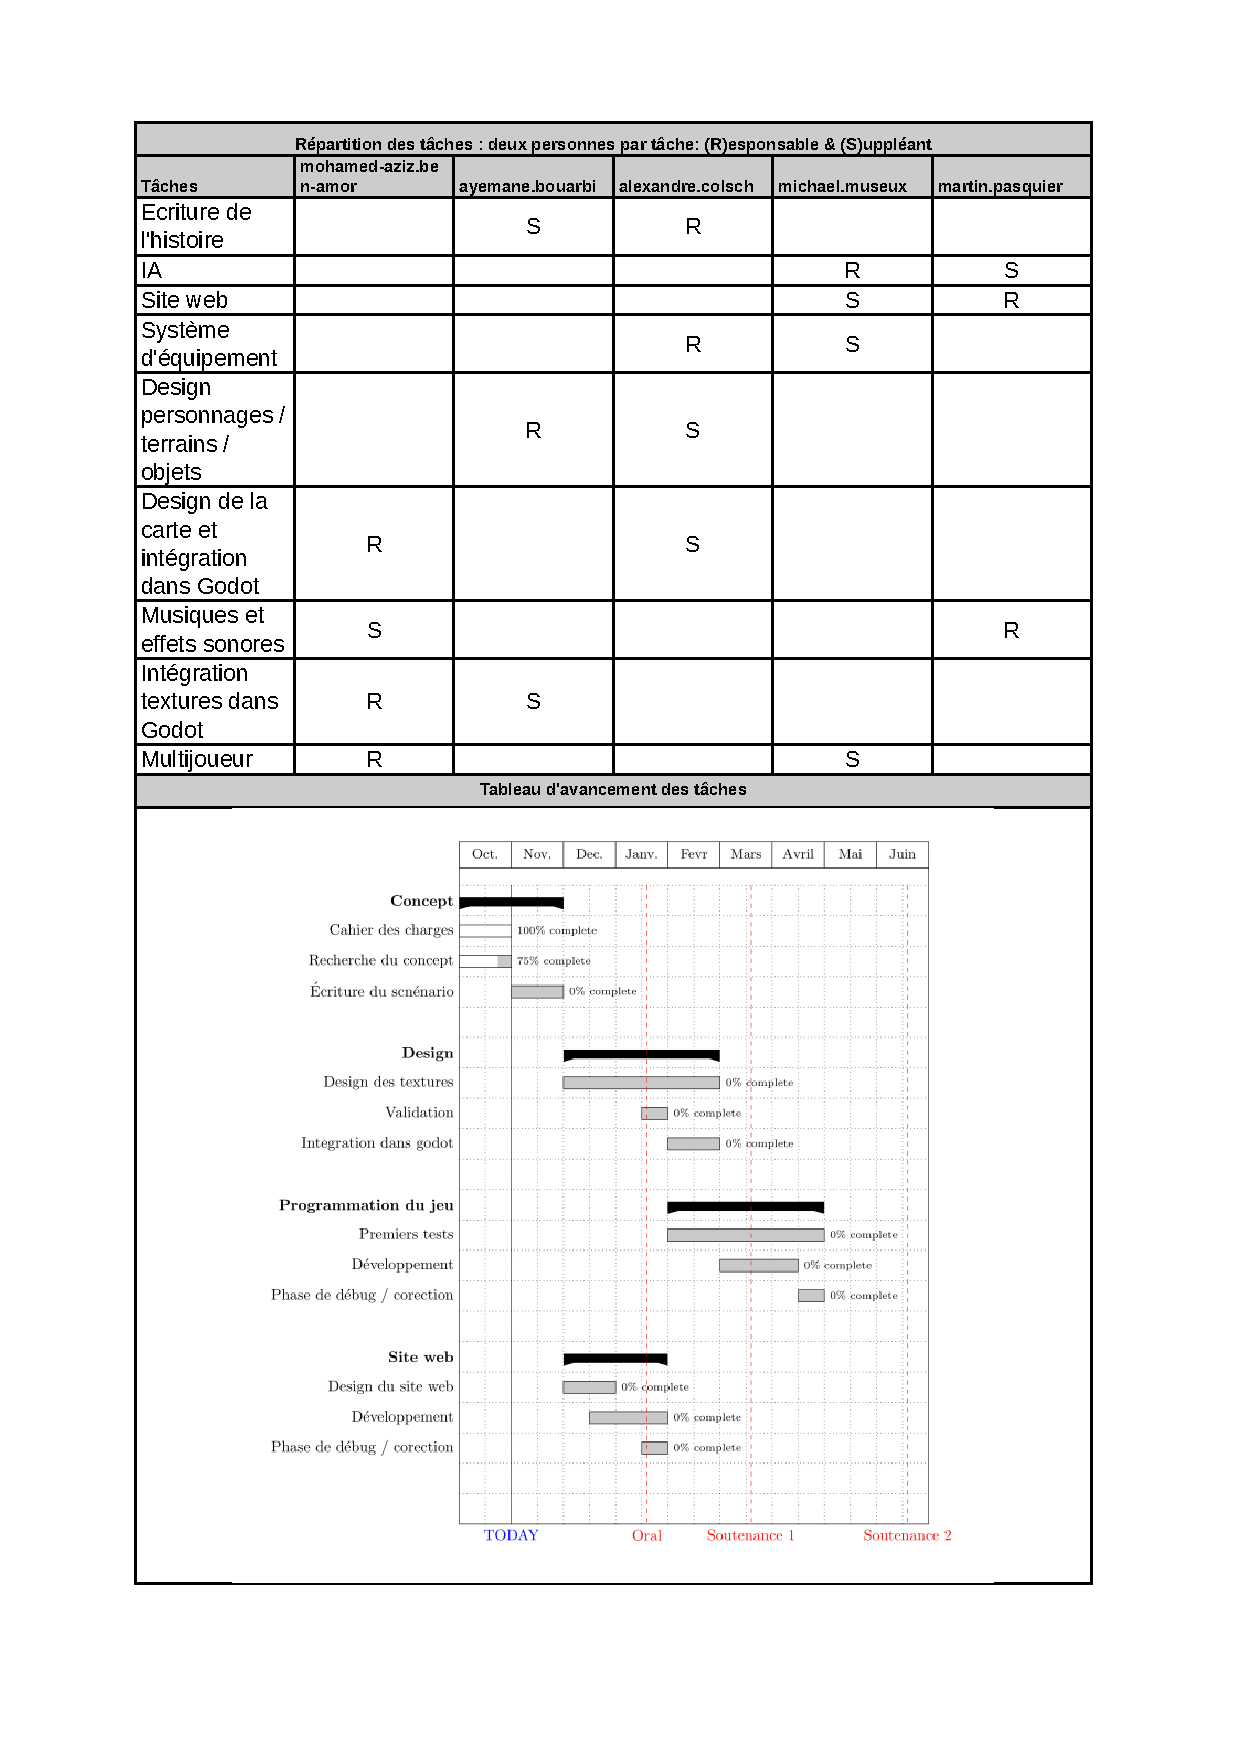
\includepdf[pages=1]{format/Technical_book-2.pdf}

\newpage
\section{Conclusion}

Ce projet a pour but de créer un jeu vidéo de rôle multijoueur avec une histoire passionnante.
Le développement de \textit{\gameName} va nous permettre d’acquérir de nouvelles compétences en C\#, en développement web, en gestion de projet et en travail d'équipe.
Notre objectif est de créer une expérience pour les joueurs, un jeu qui les rassemble et qui leur permet de s'amuser ensemble.
Explorer le monde du jeu doit être soit un plaisir pour le joueur, soit une expérience immersive et intrigante.

Dans ce cahier des charges, nous avons abordés tous les points qui définissent notre projet.
Nous avons tous des histoires différentes, des compétences différentes et des objectifs différents mais nous avons tous un point commun : nous voulons créer \textit{\gameName}.

La gestion d'un groupe de travail et d'un projet d'équipe est une compétence importante dans le monde du travail.
L'acquérir dès la première année de notre formation est donc un bon point pour notre avenir professionnel.
Il s'agit pour nous d'explorer par nous même les aspects complexes du développement de jeux vidéo, et de nous confronter aux problématiques de ce métier pendant notre formation.

Bien que des difficultés soient à prévoir, nous sommes confiants quant à la réussite de ce projet. 
Ce sera une expérience enrichissante pour nous tous et formatrice des attentes du monde professionnel.
Ce projet est aussi important dans le cadre de notre formation d'ingénieur à l'EPITA.
En effet, il constitue une première expérience de travail en équipe sur un projet de grande envergure, avec des contraintes de temps et de qualité de travail.

\subsubsection*{Perspectives d'évolution}

Durant la réalisation de ce cahier des charges, nous avons pu nous rendre compte de l'ampleur du projet.
Le développement de \textit{\gameName} est un projet ambitieux qui va nous demander beaucoup de temps et d'efforts.
C'est pourquoi nous avons pensé à plusieurs perspectives d'évolution pour le groupe.

Améliorer la jouabilité du jeu est un point important pour nous.
Nous souhaitons proposer notre jeu aux maximum de joueurs possible, c'est pourquoi nous allons le rendre disponible sur plusieurs plateformes.
En effet, Godot permet de publier le jeu sur de multiples systèmes sans trop de difficultés.

L'organisation du groupe est un point important pour la réussite du projet.
Nous avons donc décidé de prendre des décisions pour améliorer l'efficacité et la fiabilité du groupe.
Après avoir instauré une réunion hebdomadaire, nous avons décidé de demander à chaque personne du groupe un point d'avancée sur son travail.
Cela permet de savoir où en est chaque membre du groupe et de pouvoir l'aider si besoin.


\centering
\vspace*{1.5cm}

\includegraphics[width=3cm]{format/logo.png}





\end{document}
